%%%%%%%% ICML 2018 EXAMPLE LATEX SUBMISSION FILE %%%%%%%%%%%%%%%%%

\documentclass{article}

% Recommended, but optional, packages for figures and better typesetting:
\usepackage{microtype}
\usepackage{graphicx}
\usepackage{subfigure}
\usepackage{booktabs} % for professional tables

% hyperref makes hyperlinks in the resulting PDF.
% If your build breaks (sometimes temporarily if a hyperlink spans a page)
% please comment out the following usepackage line and replace
% \usepackage{icml2018} with \usepackage[nohyperref]{icml2018} above.
\usepackage{hyperref}



% Attempt to make hyperref and algorithmic work together better:
\newcommand{\theHalgorithm}{\arabic{algorithm}}
% Use the following line for the initial blind version submitted for review:
\usepackage[accepted]{icml2018}

% The \icmltitle you define below is probably too long as a header.
% Therefore, a short form for the running title is supplied here:
\icmltitlerunning{Predicting Book Genres from Their Summaries}
\graphicspath{ {./} }

\begin{document}

\twocolumn[
\icmltitle{What is this Book's Genre?}

% It is OKAY to include author information, even for blind
% submissions: the style file will automatically remove it for you
% unless you've provided the [accepted] option to the icml2018
% package.

% List of affiliations: The first argument should be a (short)
% identifier you will use later to specify author affiliations
% Academic affiliations should list Department, University, City, Region, Country
% Industry affiliations should list Company, City, Region, Country

% You can specify symbols, otherwise they are numbered in order.
% Ideally, you should not use this facility. Affiliations will be numbered
% in order of appearance and this is the preferred way.
\icmlsetsymbol{equal}{*}

\begin{icmlauthorlist}
\icmlauthor{Hakan AKYUREK}{huceng}
\icmlauthor{Sefa YURTSEVEN}{huceng}
\end{icmlauthorlist}

%\icmlaffiliation{to}{Department of Computation, University of Torontoland, Torontoland, Canada}
\icmlaffiliation{huceng}{Hacettepe University, Department of Computer Engineering}
\icmlcorrespondingauthor{}{}
% You may provide any keywords that you
% find helpful for describing your paper; these are used to populate
% the "keywords" metadata in the PDF but will not be shown in the document
\icmlkeywords{Machine Learning, BBM406}

\vskip 0.3in
]

% this must go after the closing bracket ] following \twocolumn[ ...

% This command actually creates the footnote in the first column
% listing the affiliations and the copyright notice.
% The command takes one argument, which is text to display at the start of the footnote.
% The \icmlEqualContribution command is standard text for equal contribution.
% Remove it (just {}) if you do not need this facility.

%\printAffiliationsAndNotice{}  % leave blank if no need to mention equal contribution
\printAffiliationsAndNotice{\icmlEqualContribution} % otherwise use the standard text.

\begin{abstract}
In this paper we discuss various methods for predicting a book's genre from it's summary. We experiment with CMU Book Summary dataset with 16000 book summaries along with their respective authors and multiple genres. Right now we evaluate our results considering if predicted genre is one of book's labels, but we aim to evaluate our results with multi-label evaluation metrics such as Hamming Scoring.
\end{abstract}

\section{Introduction}

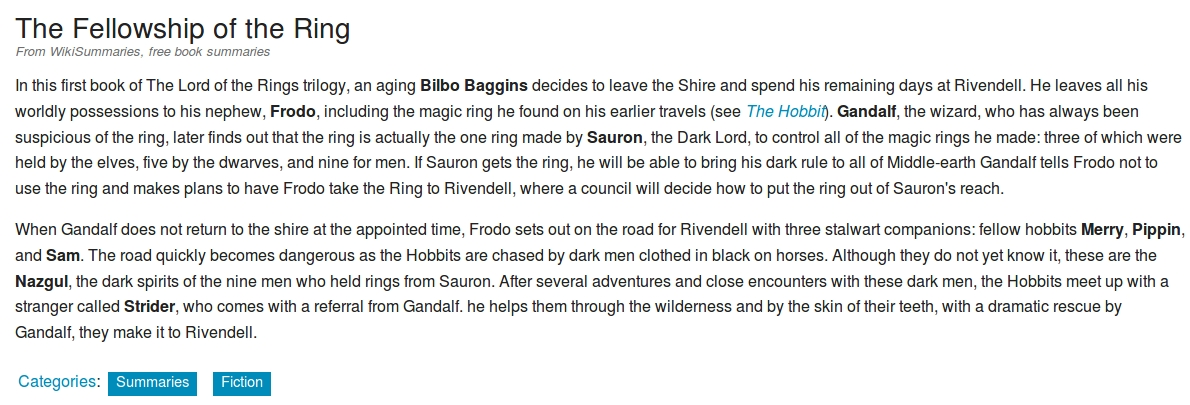
\includegraphics[width=8.5cm, height=6cm]{lotr}

Finding book genres from their summaries is a different topic that challenges us with some of the  common NLP and Machine Learning problems. The problem in question is quite challenging and as much as interesting as it requires working with a highly imbalanced multi-labelled dataset, which requires data balancing techniques and multi-label algorithms, which we couldn't find a chance to work with before.

Book genre prediction is a rather unique problem, while being a variation of a common text classification problem. It is important in cases such as: library documentation or book store database construction. Recently, many researches worked on the problem of both imbalanced datasets and multi-label text classification or multi-label classification in general. So, few algorithms have been devised for multi-label classification. Common approaches include Bayesian approach and binary approach.

In this study we came up with our own approach to multi-label classification and analysed it and are going to work with other approaches in literature about the problem in the future. We use vectorised text documents to feed our ANN and other models. The vectorised documents go through some preprocessing before being fed to a model.

It is important to note that, we started this study considering it will be a multi-class classification problem. Accordingly, we researched methods about multi-class text classification problems, so the initial results are results of our own approach.

Main contributions can be considered as such:
\begin{itemize}
\item[•] Classification of multi-label data in a single label and it's evaluation.
\item[•] Analysis of classification of multi-label data with a few models is literature.
\end{itemize}

The rest of the paper is as follows. We briefly review the related studies in Sec. 2. In Sec. 3 we describe our approach in detail. Results of experiments are discussed in Sec. 4. We discuss our conclusions in Sec. 5.

\section{Related Works}
This study \cite{ImbalancedNB} discusses handling skewed data while working with Multinomial-Naive-Bayes\cite{MNB}. But Naive-Bayes is used for comparing results by us, so we mainly studied text classification using neural networks\cite{ANN1}\cite{ANN2}.

According to imbalanced dataset problem, one can oversample\cite{resample}, under-sample\cite{resample}. Under-sampling has various methods like NearMiss, Random under sampling, Tomek link removal, and they are briefly discussed in this paper\cite{resamplep}. Oversampling methods' performance are discussed in this report\cite{over}. 

We also researched about multi-label text classification in literature. This paper\cite{movie} discusses predicting movie genres from their plot summaries using various methods and analyses their performance. Of course there is still data imbalance with our dataset\cite{ds}\cite{mli} and some researches are worked on this problem.

\section{Our Approach}
The aim of the study is to analyse various methods' and approaches' performance on classifying book genres using their summaries. Accordingly, the goal is to predict book genres as accurate as possible, again, using only their summaries. Obviously, this problem is no different than a standard text classification problem. However, working on a imbalanced dataset is what makes it different.

We believe that evaluating our results in a different manner would benefit us with more correct information about the things we do. Since many books belong to multiple genres, classifying a book to only one genre is somewhat wrong, because a book often belongs to multiple genres. We come up with two kinds of evaluations about this: 
\begin{itemize}
\item[•] Pick the class with highest probability and search it if it is one of books genres.
\item[•] Add a threshold to the outputs and pick classes with probability above that threshold instead of picking the highest one.
\end{itemize}

In this study we use a dataset[7] created from wikipedia book database. The dataset contains 16000 book information, which include publication date, author, summary, genres, name. Most books have multiple, unequal number of genres. From the dataset one can extract around 200 different book genre types. But number of books assigned to each genre is really uneven. For example a genre type has only 1 book assigned to it while another has 4000. To avoid the problems this imbalance causes we filtered our dataset to have only the top 27 genres and their books, thus leaving us with around 12000 books. In this filtered form our dataset has at least 100 books assigned to each book.

We chose ANN as our main method in the project. Simply because working with neural networks beats many other approaches in terms of performance and it is an interest of ours. If we were to compare it with a common method like NB, we could say that NN can handle word sequences and relationship between them much better than NB. We also learned that NN will perform better at relatively huger dataset. Although learning process for NN's are longer, they make it up with their better accuracy, since our aim is to get better accuracy we can say that NN's are a better choice for us.

Before our data goes into our model we do some pre-processing: removing stopwords, punctuations, lowering all characters, stemming or lemmatizing. After our data is prepared we first vectorize each input in bag of words manner, since we need to feed numerical data to our ANN model. We also use tfidf techniques to get more distinct input data. Then, we feed our input matrix to our NN. We are using keras' sequential neural network model with 'relu' activation functions. We are currently in the state of tuning hyper-parameters , but we got 63\% accuracy so far with our model.

In our ANN model we used  categorical crossentropy as loss function.

\section{Experimental Results}
We run some experiments on Naive Bayes. The accuracy scores are represented in the table below.

\begin{table}[htb]
\caption{Naive Bayes Accuracies with different methods}

\vskip 0.15in
\begin{center}
\begin{small}
\begin{sc}
\begin{tabular}{lccr}
\toprule
Experiment & Accuracy \\
\midrule
 Base                	  & 61.5\% \\
 TFidf                	  & 62.7\% \\
 Equal class priors      & 63.8\% \\
 Equal class priors-TFidf& 63.7\% \\
 Remove stopwords-TFidf  & 61.8\% \\
 Stemmed data        	  & 60.2\% \\
 Lemmatized data      	  & 60.0\% \\
 Smoothing alpha=0.03    & 56.7\% \\
 1-3 gram                & 56.5\% \\
 
\bottomrule
\end{tabular}
\end{sc}
\end{small}
\end{center}
\vskip -0.1in
\end{table}

Looking at the experiments, we can can quickly analyse a few key points. Firstly, equal class priors increase the accuracy most. From this we can easily say that our dataset is imbalanced without even checking the dataset manually. Interestingly, common preprocessing techniques of textual data do not increase and even decrease the accuracy score. We can also see that playing with some hyper-parameters in our Vectorizer and Naive Bayes classifier does not help at all and makes the model overfit the training data. Playing around with these \textbf{most accuracy we got is 64.1\%}. Currently we haven't applied any re-sampling techniques on our dataset, and we aim to try a few before switching to multi-label classification.

Unlike Naive Bayes stemming and lemmatizing increase model's performance, as they should. When we look to the activation functions sigmoid performs better than relu in terms of performance, it seems sigmoid handles text classification better than relu. With neuron count increasing in each layer model's performance seems to increase a little bit. But with a single layer of 512 neurons model directly overfits the training data, reducing accuracy to 47\%. Other than that adding a third hidden layer again made model to overfit the training data, maybe adding extra layers with less neurons can help ANN perform better than MNB. \textbf{The best accuracy we got at this point is 62.8\%}.

\begin{table}[htb]
\caption{ANN Accuracies with different methods}

\vskip 0.15in
\begin{center}
\begin{small}
\begin{sc}
\begin{tabular}{lccr}
\toprule
Experiment & Accuracy \\
\midrule
 Base-sig-sig(128n, 128n)    & 59.2\% \\
 Base-relu-relu(128n, 128n)  & 55.4\% \\
 Base-sig-sig(256n, 256n)    & 62.8\% \\
 Base-relu-relu(256n, 256n)  & 56.9\% \\
 Base-sig-sig-sig(128each)   & 55.5\% \\
 Base-relu(512n)             & 47.1\% \\
 Stemmed data                & 61.5\% \\
 Lemmatized data             & 60.7\% \\
 Stemmed and Lemmatized data & 61.3\% \\
\bottomrule
\end{tabular}
\end{sc}
\end{small}
\end{center}
\vskip -0.15in
\end{table}

\section{Conclusions}
Before switching to multi-label classification for sure, we approached this classification problem from a different angle based on our knowledge. We approached this as a multi-class classification problem. However, we aim to work on multi-label classification from here on out.

As we mentioned this is a multi-label classification problem in origin. We came to a conclusion about that after studying the confusion matrix below.

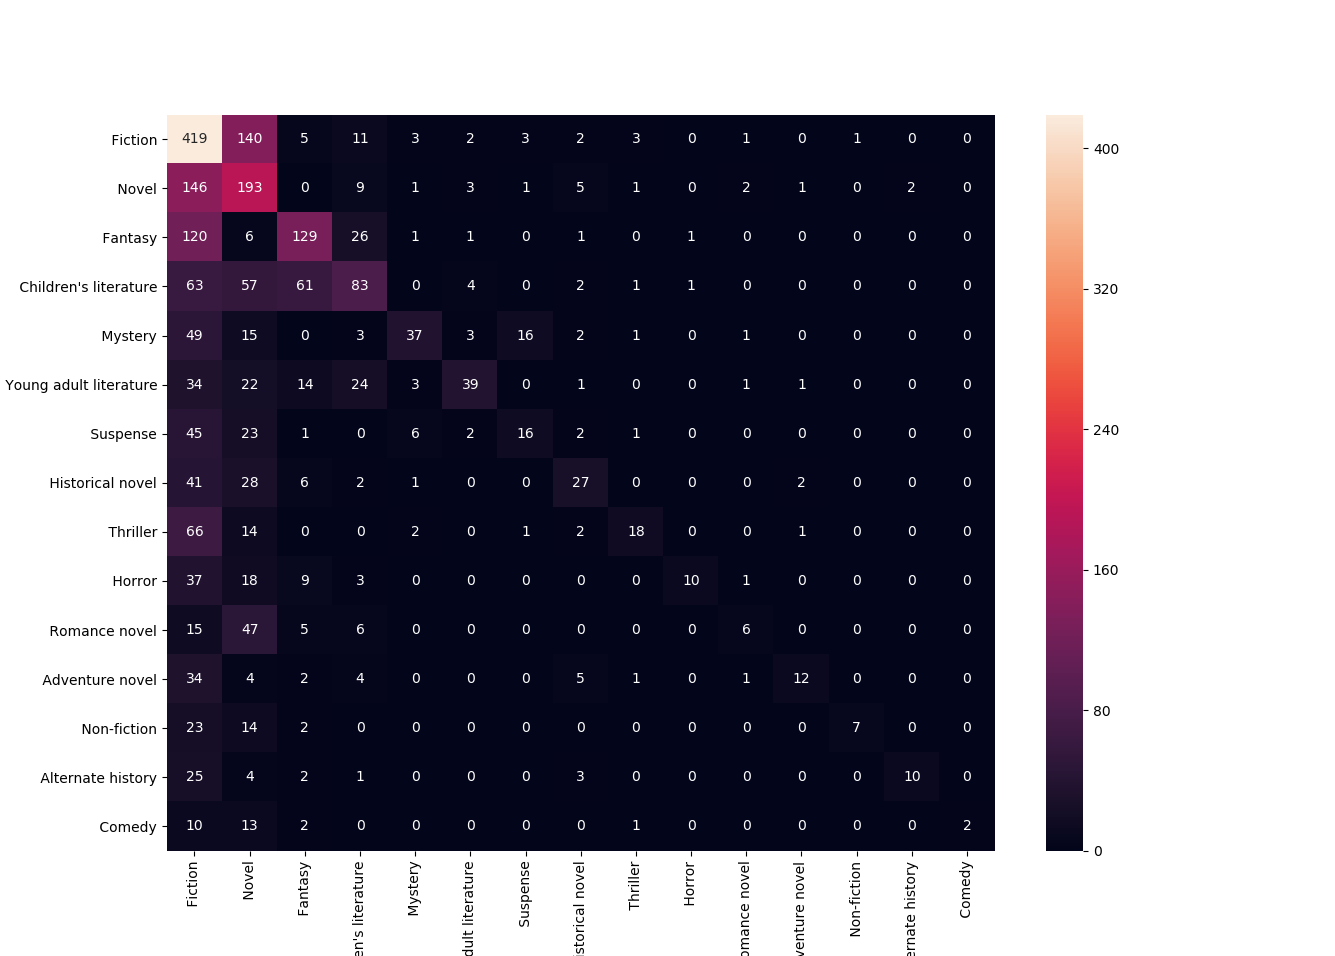
\includegraphics[width=10cm, height=8.5cm]{conf_matrix}

From looking to this matrix, we can see that there is something seriously wrong with the top most 4 classes. It can be seen that around half of the documents are misclassified in these classes. After looking to dataset more closely we noticed that some of the misclassified documents actually also belong to the classes our model classified. This was the trigger that made us research more on this topic and learn about multi-label classification.

We run many experiments on both Naive Bayes and ANN models. Both seemed to perform similar at best. We believe that it is because we chose to work with ANN's instead of RNN's or CNN's and our ANN model needs more hyper-parameter tuning. Highest accuracies of both models are represented in the table below.

\begin{table}[htb]
\caption{Best classification accuracies for Naive Bayes and ANN.}
\label{sample-table}
\vskip 0.15in
\begin{center}
\begin{small}
\begin{sc}
\begin{tabular}{lccr}
\toprule
Method & Best Accuracy \\
\midrule
Naive Bayes    & 63.8\% \\
ANN            & 62.8\%\\
\bottomrule
\end{tabular}
\end{sc}
\end{small}
\end{center}
\vskip -0.1in
\end{table}

Nevertheless, this isn't what we hoped for. We though artificial neural could easily perform batter than Naive Bayes. Maybe ANN is not the correct NN for text classification, we read RNN and CNN perform really well with text classification. Switching to them doesn't seem that illogical at this point.

% 1 http://people.csail.mit.edu/jrennie/papers/icml03-nb.pdf
% 2 https://link.springer.com/content/pdf/10.1007%2F0-387-24049-7_12.pdf
% 3 http://citeseerx.ist.psu.edu/viewdoc/download?doi=10.1.1.473.5982&rep=rep1&type=pdf
% 4 https://en.wikipedia.org/wiki/Oversampling_and_undersampling_in_data_analysis
% 5 https://arxiv.org/pdf/1608.06048.pdf
% 6 https://run.unl.pt/bitstream/10362/31307/1/TEGI0396.pdf
% 7 http://www.cs.cmu.edu/~dbamman/booksummaries.html
% 8 https://www.researchgate.net/publication/%322517980_Predicting_Movie_Genres_Based_on_Plot_Summaries
% 9 https://sci2s.ugr.es/sites/default/files/ficherosPublicaciones/1790_2015-Neuro-Charte-%MultiLabel_Imbalanced.pdf
%10 https://minerva.leeds.ac.uk/bbcswebdav/orgs/SCH_Computing/FYProj/reports/1415/MURRAY.pdf
\bibliography{Progress Report}
\bibliographystyle{icml2018}

\end{document}


% This document was modified from the file originally made available by
% Pat Langley and Andrea Danyluk for ICML-2K. This version was created
% by Iain Murray in 2018. It was modified from a version from Dan Roy in
% 2017, which was based on a version from Lise Getoor and Tobias
% Scheffer, which was slightly modified from the 2010 version by
% Thorsten Joachims & Johannes Fuernkranz, slightly modified from the
% 2009 version by Kiri Wagstaff and Sam Roweis's 2008 version, which is
% slightly modified from Prasad Tadepalli's 2007 version which is a
% lightly changed version of the previous year's version by Andrew
% Moore, which was in turn edited from those of Kristian Kersting and
% Codrina Lauth. Alex Smola contributed to the algorithmic style files.
